\usepackage{listings}%  A simple AAU report template.
%  2015-05-08 v. 1.2.0
%  Copyright 2010-2015 by Jesper Kjær Nielsen <jkn@es.aau.dk>
%
%  This is free software: you can redistribute it and/or modify
%  it under the terms of the GNU General Public License as published by
%  the Free Software Foundation, either version 3 of the License, or
%  (at your option) any later version.
%
%  This is distributed in the hope that it will be useful,
%  but WITHOUT ANY WARRANTY; without even the implied warranty of
%  MERCHANTABILITY or FITNESS FOR A PARTICULAR PURPOSE.  See the
%  GNU General Public License for more details.
%
%  You can find the GNU General Public License at <http://www.gnu.org/licenses/>.
%
%  A simple AAU report template.
%  2015-05-08 v. 1.2.0
%  Copyright 2010-2015 by Jesper Kjær Nielsen <jkn@es.aau.dk>
%
%  This is free software: you can redistribute it and/or modify
%  it under the terms of the GNU General Public License as published by
%  the Free Software Foundation, either version 3 of the License, or
%  (at your option) any later version.
%
%  This is distributed in the hope that it will be useful,
%  but WITHOUT ANY WARRANTY; without even the implied warranty of
%  MERCHANTABILITY or FITNESS FOR A PARTICULAR PURPOSE.  See the
%  GNU General Public License for more details.
%
%  You can find the GNU General Public License at <http://www.gnu.org/licenses/>.
%
\documentclass[11pt,a4paper,openany]{report}
%%%%%%%%%%%%%%%%%%%%%%%%%%%%%%%%%%%%%%%%%%%%%%%%
% Language, Encoding and Fonts
% http://en.wikibooks.org/wiki/LaTeX/Internationalization
%%%%%%%%%%%%%%%%%%%%%%%%%%%%%%%%%%%%%%%%%%%%%%%%
% Select encoding of your inputs. Depends on
% your operating system and its default input
% encoding. Typically, you should use
%   Linux  : utf8 (most modern Linux distributions)
%            latin1 
%   Windows: ansinew
%            latin1 (works in most cases)
%   Mac    : applemac
% Notice that you can manually change the input
% encoding of your files by selecting "save as"
% an select the desired input encoding. 
\usepackage[utf8]{inputenc}
% Make latex understand and use the typographic
% rules of the language used in the document.
\usepackage[danish,english]{babel}
% Use the palatino font
\usepackage[sc]{mathpazo}
\linespread{1.05}         % Palatino needs more leading (space between lines)
% Choose the font encoding
\usepackage[T1]{fontenc}
%%%%%%%%%%%%%%%%%%%%%%%%%%%%%%%%%%%%%%%%%%%%%%%%
% Graphics and Tables
% http://en.wikibooks.org/wiki/LaTeX/Importing_Graphics
% http://en.wikibooks.org/wiki/LaTeX/Tables
% http://en.wikibooks.org/wiki/LaTeX/Colors
%%%%%%%%%%%%%%%%%%%%%%%%%%%%%%%%%%%%%%%%%%%%%%%%
% load a colour package
\usepackage{xcolor}
\definecolor{aaublue}{RGB}{33,26,82}% dark blue
% The standard graphics inclusion package
\usepackage{graphicx}
% Set up how figure and table captions are displayed
\usepackage{caption}
\captionsetup{%
  font=footnotesize,% set font size to footnotesize
  labelfont=bf % bold label (e.g., Figure 3.2) font
}
% Make the standard latex tables look so much better
\usepackage{array,booktabs}
% Enable the use of frames around, e.g., theorems
% The framed package is used in the example environment
\usepackage{framed}

%%%%%%%%%%%%%%%%%%%%%%%%%%%%%%%%%%%%%%%%%%%%%%%%
% Mathematics
% http://en.wikibooks.org/wiki/LaTeX/Mathematics
%%%%%%%%%%%%%%%%%%%%%%%%%%%%%%%%%%%%%%%%%%%%%%%%
% Defines new environments such as equation,
% align and split 
\usepackage{amsmath}
% Adds new math symbols
\usepackage{amssymb}
% Use theorems in your document
% The ntheorem package is also used for the example environment
% When using thmmarks, amsmath must be an option as well. Otherwise \eqref doesn't work anymore.
\usepackage[framed,amsmath,thmmarks]{ntheorem}

%%%%%%%%%%%%%%%%%%%%%%%%%%%%%%%%%%%%%%%%%%%%%%%%
% Page Layout
% http://en.wikibooks.org/wiki/LaTeX/Page_Layout
%%%%%%%%%%%%%%%%%%%%%%%%%%%%%%%%%%%%%%%%%%%%%%%%
% Change margins, papersize, etc of the document
\usepackage[
  inner=28mm,% left margin
  outer=41mm,% right margin
  ]{geometry}
% Modify how \chapter, \section, etc. look
% The titlesec package is very configureable
\usepackage{titlesec}
\titleformat{\chapter}[display]{\normalfont\huge\bfseries}{\chaptertitlename\ \thechapter}{20pt}{\Huge}
\titleformat*{\section}{\normalfont\Large\bfseries}
\titleformat*{\subsection}{\normalfont\large\bfseries}
\titleformat*{\subsubsection}{\normalfont\normalsize\bfseries}
%\titleformat*{\paragraph}{\normalfont\normalsize\bfseries}
%\titleformat*{\subparagraph}{\normalfont\normalsize\bfseries}

% Clear empty pages between chapters
\let\origdoublepage\cleardoublepage
\newcommand{\clearemptydoublepage}{%
  \clearpage
  {\pagestyle{empty}\origdoublepage}%
}
\let\cleardoublepage\clearemptydoublepage

% Change the headers and footers
\usepackage{fancyhdr}
\pagestyle{fancy}
\fancyhf{} %delete everything
\renewcommand{\headrulewidth}{0pt} %remove the horizontal line in the header
\fancyhead[RE]{\small\nouppercase\leftmark} %even page - chapter title
\fancyhead[LO]{\small\nouppercase\rightmark} %uneven page - section title
\fancyhead[LE,RO]{\thepage} %page number on all pages
% Do not stretch the content of a page. Instead,
% insert white space at the bottom of the page
\raggedbottom
% Enable arithmetics with length. Useful when
% typesetting the layout.
\usepackage{calc}

%%%%%%%%%%%%%%%%%%%%%%%%%%%%%%%%%%%%%%%%%%%%%%%%
% Bibliography
% http://en.wikibooks.org/wiki/LaTeX/Bibliography_Management
%%%%%%%%%%%%%%%%%%%%%%%%%%%%%%%%%%%%%%%%%%%%%%%%
\usepackage[backend=biber,
  bibencoding=utf8
  ]{biblatex}
\addbibresource{bib/mybib.bib}

%%%%%%%%%%%%%%%%%%%%%%%%%%%%%%%%%%%%%%%%%%%%%%%%
% Misc
%%%%%%%%%%%%%%%%%%%%%%%%%%%%%%%%%%%%%%%%%%%%%%%%
% Add bibliography and index to the table of
% contents
\usepackage[nottoc]{tocbibind}
% Add the command \pageref{LastPage} which refers to the
% page number of the last page
\usepackage{lastpage}
% Add todo notes in the margin of the document
\usepackage[
%  disable, %turn off todonotes
  colorinlistoftodos, %enable a coloured square in the list of todos
  textwidth=\marginparwidth, %set the width of the todonotes
  textsize=scriptsize, %size of the text in the todonotes
  ]{todonotes}

%%%%%%%%%%%%%%%%%%%%%%%%%%%%%%%%%%%%%%%%%%%%%%%%
% Hyperlinks
% http://en.wikibooks.org/wiki/LaTeX/Hyperlinks
%%%%%%%%%%%%%%%%%%%%%%%%%%%%%%%%%%%%%%%%%%%%%%%%
% Enable hyperlinks and insert info into the pdf
% file. Hypperref should be loaded as one of the 
% last packages
\usepackage{hyperref}
\hypersetup{%
	pdfpagelabels=true,%
	plainpages=false,%
	pdfauthor={Author(s)},%
	pdftitle={Title},%
	pdfsubject={Subject},%
	bookmarksnumbered=true,%
	colorlinks=false,%
	citecolor=black,%
	filecolor=black,%
	linkcolor=black,% you should probably change this to black before printing
	urlcolor=black,%
	pdfstartview=FitH%
}

\usepackage{listings}

\definecolor{codegreen}{rgb}{0,0.6,0}
\definecolor{codegray}{rgb}{0.5,0.5,0.5}
\definecolor{codepurple}{rgb}{0.58,0,0.82}
\definecolor{backcolour}{rgb}{0.95,0.95,0.92}

\lstdefinelanguage{json}{
    basicstyle=\normalfont\ttfamily,
    numbers=left,
    numberstyle=\scriptsize,
    stepnumber=1,
    numbersep=8pt,
    showstringspaces=false,
    breaklines=true,
    frame=lines,
    backgroundcolor=\color{background},
    literate=
     *{0}{{{\color{numb}0}}}{1}
      {1}{{{\color{numb}1}}}{1}
      {2}{{{\color{numb}2}}}{1}
      {3}{{{\color{numb}3}}}{1}
      {4}{{{\color{numb}4}}}{1}
      {5}{{{\color{numb}5}}}{1}
      {6}{{{\color{numb}6}}}{1}
      {7}{{{\color{numb}7}}}{1}
      {8}{{{\color{numb}8}}}{1}
      {9}{{{\color{numb}9}}}{1}
      {:}{{{\color{punct}{:}}}}{1}
      {,}{{{\color{punct}{,}}}}{1}
      {\{}{{{\color{delim}{\{}}}}{1}
      {\}}{{{\color{delim}{\}}}}}{1}
      {[}{{{\color{delim}{[}}}}{1}
      {]}{{{\color{delim}{]}}}}{1},
}

\lstdefinestyle{python}{
    backgroundcolor=\color{backcolour},
    commentstyle=\color{codegreen},
    keywordstyle=\color{magenta},
    numberstyle=\tiny\color{codegray},
    stringstyle=\color{codepurple},
    basicstyle=\ttfamily\footnotesize,
    breakatwhitespace=false,
    breaklines=true,
    captionpos=b,
    keepspaces=true,
    numbers=left,
    numbersep=5pt,
    showspaces=false,
    showstringspaces=false,
    showtabs=false,
    tabsize=2
}

\lstset{style=python}



\colorlet{punct}{red!60!black}
\definecolor{background}{HTML}{EEEEEE}
\definecolor{delim}{RGB}{20,105,176}
\colorlet{numb}{magenta!60!black}

\usepackage{bchart}

\usepackage{float}% package inclusion and set up of the document
% see, e.g., http://en.wikibooks.org/wiki/LaTeX/Formatting#Hyphenation
% for more information on word hyphenation
\hyphenation{ex-am-ple hy-phen-a-tion short}
\hyphenation{long la-tex}%
%  A simple AAU report template.
%  2015-05-08 v. 1.2.0
%  Copyright 2010-2015 by Jesper Kjær Nielsen <jkn@es.aau.dk>
%
%  This is free software: you can redistribute it and/or modify
%  it under the terms of the GNU General Public License as published by
%  the Free Software Foundation, either version 3 of the License, or
%  (at your option) any later version.
%
%  This is distributed in the hope that it will be useful,
%  but WITHOUT ANY WARRANTY; without even the implied warranty of
%  MERCHANTABILITY or FITNESS FOR A PARTICULAR PURPOSE.  See the
%  GNU General Public License for more details.
%
%  You can find the GNU General Public License at <http://www.gnu.org/licenses/>.
%
%
%
% see, e.g., http://en.wikibooks.org/wiki/LaTeX/Customizing_LaTeX#New_commands
% for more information on how to create macros

%%%%%%%%%%%%%%%%%%%%%%%%%%%%%%%%%%%%%%%%%%%%%%%%
% Macros for the titlepage
%%%%%%%%%%%%%%%%%%%%%%%%%%%%%%%%%%%%%%%%%%%%%%%%
%Creates the aau titlepage
\newcommand{\aautitlepage}[3]{%
  {
    %set up various length
    \ifx\titlepageleftcolumnwidth\undefined
      \newlength{\titlepageleftcolumnwidth}
      \newlength{\titlepagerightcolumnwidth}
    \fi
    \setlength{\titlepageleftcolumnwidth}{0.5\textwidth-\tabcolsep}
    \setlength{\titlepagerightcolumnwidth}{\textwidth-2\tabcolsep-\titlepageleftcolumnwidth}
    %create title page
    \thispagestyle{empty}
    \noindent%
    \begin{tabular}{@{}ll@{}}
      \parbox{\titlepageleftcolumnwidth}{
        \iflanguage{danish}{%
          
\includegraphics[width=\titlepageleftcolumnwidth]{figures/aau_logo_da}
        }{%
          
\includegraphics[width=\titlepageleftcolumnwidth]{figures/aau_logo_en}
        }
      } &
      \parbox{\titlepagerightcolumnwidth}{\raggedleft\sf\small
        #2
      }\bigskip\\
       #1 &
      \parbox[t]{\titlepagerightcolumnwidth}{%
      \textbf{Abstract:}\bigskip\par
        \fbox{\parbox{\titlepagerightcolumnwidth-2\fboxsep-2\fboxrule}{%
          #3
        }}
      }\\
    \end{tabular}
    \vfill
    \iflanguage{danish}{%
      \noindent{\footnotesize\emph{Rapportens indhold er frit tilgængeligt, men offentliggørelse (med kildeangivelse) må kun ske efter aftale med forfatterne.}}
    }{%
      \noindent{\footnotesize\emph{The content of this report is freely available, but publication (with reference) may only be pursued due to agreement with the author.}}
    }
    \clearpage
  }
}

%Create english project info
\newcommand{\englishprojectinfo}[8]{%
  \parbox[t]{\titlepageleftcolumnwidth}{
    \textbf{Title:}\\ #1\bigskip\par
    \textbf{Theme:}\\ #2\bigskip\par
    \textbf{Project Period:}\\ #3\bigskip\par
    \textbf{Project Group:}\\ #4\bigskip\par
    \textbf{Participant(s):}\\ #5\bigskip\par
    \textbf{Supervisor(s):}\\ #6\bigskip\par
    \textbf{Copies:} #7\bigskip\par
    \textbf{Page Numbers:} \pageref{LastPage}\bigskip\par
    \textbf{Date of Completion:}\\ #8
  }
}

%Create danish project info
\newcommand{\danishprojectinfo}[8]{%
  \parbox[t]{\titlepageleftcolumnwidth}{
    \textbf{Titel:}\\ #1\bigskip\par
    \textbf{Tema:}\\ #2\bigskip\par
    \textbf{Projektperiode:}\\ #3\bigskip\par
    \textbf{Projektgruppe:}\\ #4\bigskip\par
    \textbf{Deltager(e):}\\ #5\bigskip\par
    \textbf{Vejleder(e):}\\ #6\bigskip\par
    \textbf{Oplagstal:} #7\bigskip\par
    \textbf{Sidetal:} \pageref{LastPage}\bigskip\par
    \textbf{Afleveringsdato:}\\ #8
  }
}

%%%%%%%%%%%%%%%%%%%%%%%%%%%%%%%%%%%%%%%%%%%%%%%%
% An example environment
%%%%%%%%%%%%%%%%%%%%%%%%%%%%%%%%%%%%%%%%%%%%%%%%
\theoremheaderfont{\normalfont\bfseries}
\theorembodyfont{\normalfont}
\theoremstyle{break}
\def\theoremframecommand{{\color{gray!50}\vrule width 5pt \hspace{5pt}}}
\newshadedtheorem{exa}{Example}[chapter]
\newenvironment{example}[1]{%
		\begin{exa}[#1]
}{%
		\end{exa}
}% my new macros

\begin{document}
%frontmatter
\pagestyle{empty} %disable headers and footers
\pagenumbering{roman} %use roman page numbering in the frontmatter
%  A simple AAU report template.
%  2015-05-08 v. 1.2.0
%  Copyright 2010-2015 by Jesper Kjær Nielsen <jkn@es.aau.dk>
%
%  This is free software: you can redistribute it and/or modify
%  it under the terms of the GNU General Public License as published by
%  the Free Software Foundation, either version 3 of the License, or
%  (at your option) any later version.
%
%  This is distributed in the hope that it will be useful,
%  but WITHOUT ANY WARRANTY; without even the implied warranty of
%  MERCHANTABILITY or FITNESS FOR A PARTICULAR PURPOSE.  See the
%  GNU General Public License for more details.
%
%  You can find the GNU General Public License at <http://www.gnu.org/licenses/>.
%
\pdfbookmark[0]{Front page}{label:frontpage}%
\begin{titlepage}
  \addtolength{\hoffset}{0.5\evensidemargin-0.5\oddsidemargin} %set equal margins on the frontpage - remove this line if you want default margins
  \noindent%
  \begin{tabular}{@{}p{\textwidth}@{}}
    \toprule[2pt]
    \midrule
    \vspace{0.2cm}
    \begin{center}
    \Huge{\textbf{
        Improving Energy Efficiency in Python Development
    }}
    \end{center}
%    \begin{center}
%      \Large{
%        - Secure, Scalable and Useful Systems -
%      }
%    \end{center}
    \vspace{0.2cm}\\
    \midrule
    \toprule[2pt]
  \end{tabular}
  \vspace{4 cm}
  \begin{center}
    {\large
      Project Report%Insert document type (e.g., Project Report)
    }\\
    \vspace{0.2cm}
    {\Large
      Group cs-22-it-7-02
    }
  \end{center}
  \vfill
  \begin{center}
  Aalborg University\\
  Department of Computer Science
  \end{center}
\end{titlepage}
\clearpage
\thispagestyle{empty}
{\small
\strut\vfill % push the content to the bottom of the page
\noindent Copyright \copyright{} Aalborg University 2022
}
\clearpage
\pdfbookmark[0]{English title page}{label:titlepage_en}
\aautitlepage{%
    \englishprojectinfo{
        Leveraging performance profiling to increase energy efficiency in python applications %title
    }{%
        Scientific Theme %theme
    }{%
        Fall Semester 2022 %project period
    }{%
        cs-23-it-9 % project group
    }{%
    %list of group members
        Martinus Nel
    }{%
    %list of supervisors
        Bent Thomsen\\
    }{%
        1 % number of printed copies
    }{%
        \today % date of completion
    }%
}{%department and address
    \textbf{Department of Computer Science}\\
    Selma Lagerløfs Vej 300\\
    \href{http://www.cs.aau.dk/}{http://www.cs.aau.dk/}
}
{% the abstract
This report aims to tackle the issue of energy usage in python programs by exploratively studying methods for energy
profiling that developers may use to identify energy inefficient patterns in their applications.
}
\pdfbookmark[0]{Contents}{label:contents}
\pagestyle{fancy} %enable headers and footers again
\tableofcontents
%mainmatter
\pagenumbering{arabic} %use arabic page numbering in the mainmatter
\chapter{Introduction}\label{ch:introduction}

\section{Problem Statement}\label{sec:problem-statement}
\subsection{Context}\label{subsec:context}
Energy usage is a growing concern of the computing industry\cite{FrontierEnergyUsage,HistoricalComputingEnergyTrends},
with Python being a widely used language\cite{TIOBE}, it is a prime candidate for energy optimisation.

Energy optimisation has incentivised approach in several computing sectors, including but not limited to server hosting
and mobile technology.

Data centres account for a significant portion of global electricity demand\cite{IEADataCentres}, which presents a
promising avenue for reducing costs of long-term running services in an effort to reduce such
costs\cite{KIOCostsOfDataCentre, AssetSpireDataCosts}.

Similarly, mobile devices require limited batteries to operate, leading to a rather obvious incentive to optimise their
energy usage for longer uptime\cite{SmartPhoneFeatures}.

\subsection{Issue}\label{subsec:issue}
Surveys on conventional knowledge on energy consumption show a general lack of understanding for avenues to improving
power saving\cite{EnergyConsumptionKnowledge}, this means that even if developers choose to optimise their code for
energy efficiency, they may not know how to do so.
This issue is exacerbated by the opacity of modern proprietary hardware, and the layers of abstraction that modern
computers operate on - leading to a lack of understanding of the energy costs of specific operations.

These issues are not unique to energy optimisation, and the general approach is to target general abstract concepts
that are known to create inefficiencies, such as memory management, caching, and system calls.

The concept that this report hinges on is the fact that performance profiling is relatively a lot easier, as there
are more readily available system agnostic tools that simply measure the time taken for a specific operation to
execute.
This is in contrast to energy profiling, which requires system level tools or physical hardware to measure the energy
readings.
Developers who want to measure the energy profile of their system must find and implement such tools which require
knowledge of the system that the software is running on, information which may not even be readily accessible in
situations such as automated testing or cloud computing.


In summary, while both performance and energy profiling have their own challenges, performance profiling is more
accessible and easier to implement than energy profiling.

\subsection{Objectives}\label{subsec:objectives}
The objective of this report is to study the relationship of Python performance against its energy usage, with the goal
of leveraging performance profiling to predict the energy profile of a Python application.
To do this, we will have to find patterns that affect performance and energy in consistent ratios, such as specific
system calls, memory interactions, or higher level concepts.
Furthermore, we must test that these patterns scale, as specific concepts involving memory management and caching may
require more advanced approaches to make accurate predictions.

\begin{itemize}
 \item How does the performance of a Python application relate to its energy usage?
 \item What techniques are required to accurately infer the energy profile of a Python application?
\end{itemize}


\section{Related Work}\label{sec:related-work}
\subsubsection{Scaphandre}
Scaphandre\cite{Scaphandre} is a tool that is designed to monitor the energy usage of a system, similar to the purpose
of this report they seek to ``\textit{enable the tech industry to shift towards more sustainability}''.
As of the writing of this report, Scaphandre has had updates are recent as 4 months ago, and 1.5k stars on GitHub, which
are good indicators of a healthy project.


\section{Performance Profiling}\label{sec:performance-profiling}
This section will explore accepted ways to profile the speed of python applications.
Microsoft Visual Studio recognizes three forms of profiling: sampling, instrumentation, and
tracing\cite{MicrosoftProfilingTechniques}.
Profiling is a balance, as the more detailed the profiling, the more overhead is introduced to the script, in this
section we will explore all the aforementioned methods of profiling, and find the most appropriate
balance between detail and overhead.

\subsubsection{Bash Time}\label{subsubsec:bash_time}
Assuming the script is being run in a bash terminal, the time command\cite{BashTime} is a standard
simple approach to finding execution time; as per the documentation this outputs 3 values: real, user, and sys time.
Real time refers to the total time taken for the script to execute, user time refers to the time spent executing
instructions on the CPU in user space, while sys time refers to the time spent executing calls in kernel space with
elevated privileges.
This is immediately more useful than a regular clock approach, as it gives us insight into the execution time at
different levels of processing.
The bash time function returns results in milliseconds, with both user and sys time being translated from clock ticks
within the CPU - this makes it difficult to judge the accuracy of such measurements, as ``\textit{the value of HZ varies
across kernel versions and hardware platforms}''\cite{BashTimeClock}, for the purpose of this report we will assume it is
sufficient.
Lastly, as the timer is not connected to the script being tested, there is no way to create a profiler that can locate
exact points of inefficiency, simply indicate that they exist - this can be partially circumvented by creating
profiles for units of code that can be applied using static profilers.

\begin{figure}[H]
    \centering
    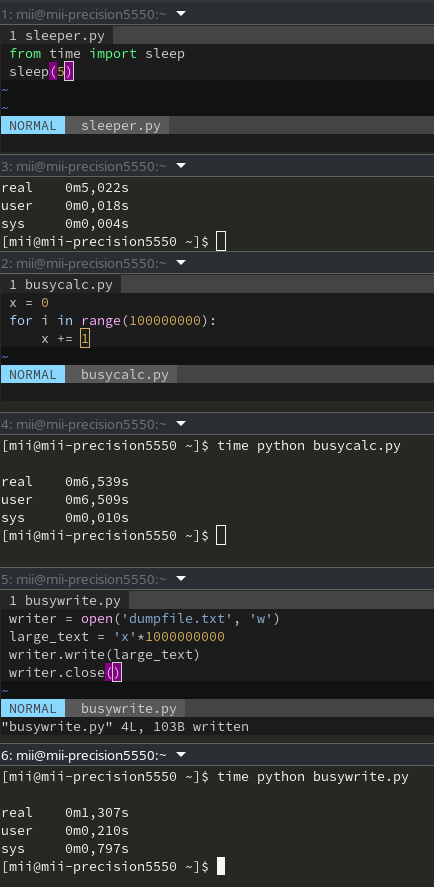
\includegraphics[width=8cm]{figures/introduction/bashtime}
    \caption{Three examples of python scripts being run in bash with time, each script maximises a different aspect of
    time - a sleep will increase overall time without increasing user or sys time; a CPU bound script will increase user
    time; and a script that waits for IO will increase sys time.}
    \label{fig:bash_time}
\end{figure}

\subsubsection{Perf}
Perf is a complex Linux tool designed to collect a myriad of different events, for this section we will focus on the
\textit{record} and \textit{report} functionality, which gathers samples of the \texit{cycles} event, this compiled 
information can be displayed as a report with various different tools, such as the gecko tool displayed in
fig\ref{fig:perf_gecko}.
Perf has the advantage of (if enabled) describing the entire system in its report, which can be useful to ascertain
whether the script is being affected by other processes, or causing extra load not accounted for in the script.

\begin{figure}[H]
    \centering
    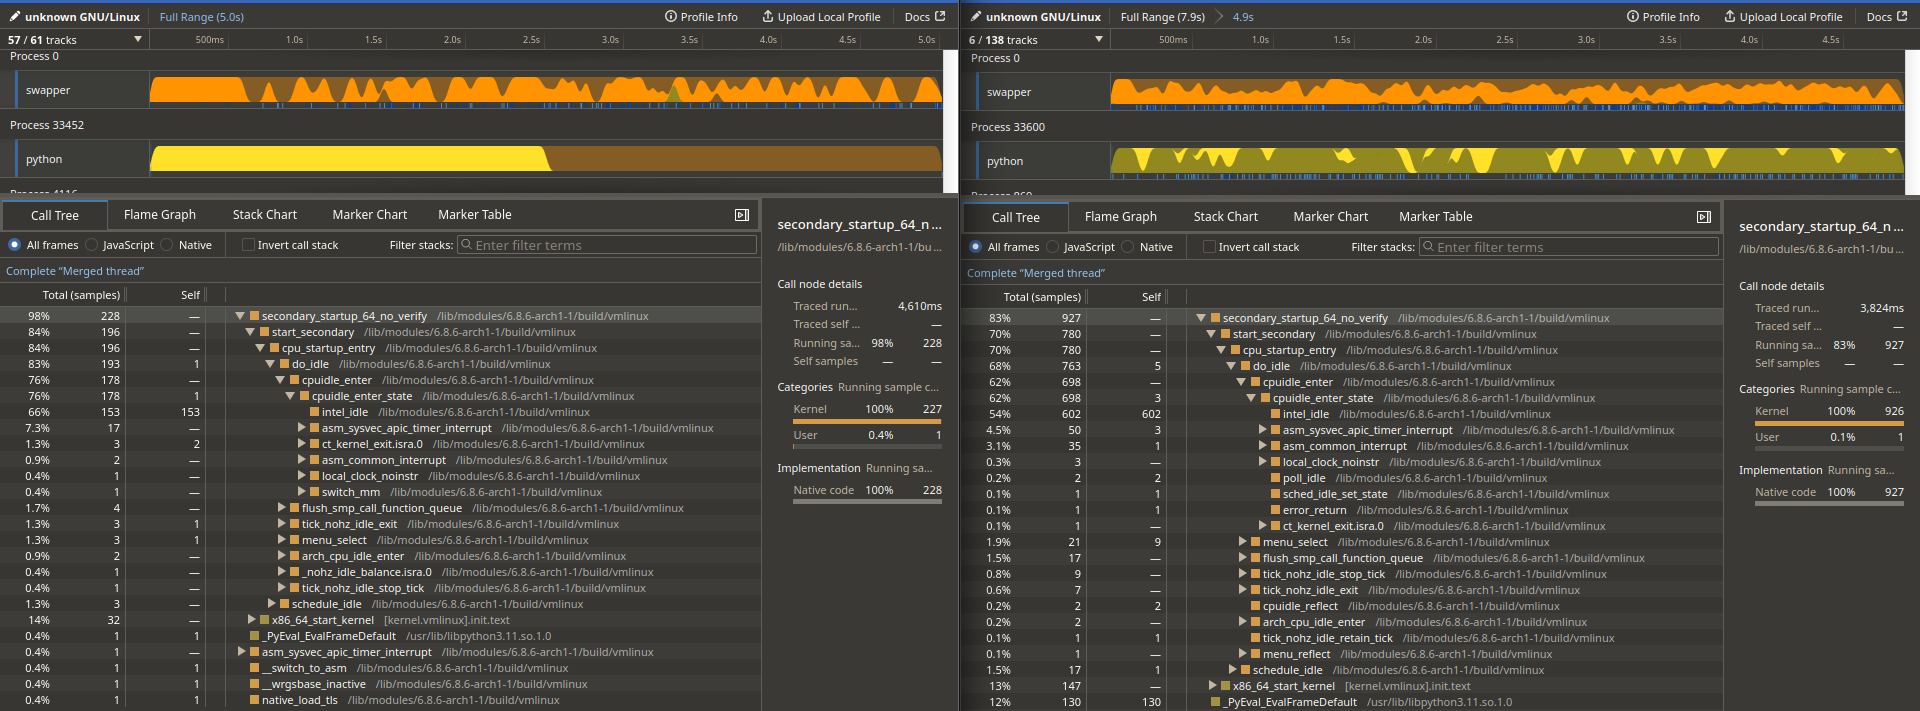
\includegraphics[width=15cm]{figures/introduction/perf_gecko_sleep_vs_calc}
    \caption{Comparing a python script that sleeps for 5 seconds (left) to the busy calc script
    from~\ref{subsubsec:bash_time} (right) note the increased amount of samples for busycalc, which may be used to
    predict its increased load}
    \label{fig:perf_gecko}
\end{figure}

\subsubsection{Python Profiler}
The python profiler\cite{PythonProfiler} is a standard tool for profiling python scripts, it improves on bash time by
providing information on the time within each call of the script, allowing for a more granular understanding of what
might be causing performance bottlenecks.
As per the documentation, the timer is limited by the underlying clock rate (1ms) - additionally due to the time between
an event and the call for the clock state can introduce inaccuracies for calls that execute many times in a short
period.
The python profiler is split into two parts, the cProfile and profile modules, the cProfile module is a C extension with
minimal overhead that is intended for our use-case, while the profile module is a pure python implementation that is
designed to be more approachable for tasks such as creating extensions - for our purposes we will focus on cProfile.
While the python profiler is a powerful tool, it is not without drawbacks, as calls themselves can be nebulous, FIGURE
shows how the previously created \textit(busycalc) script has no definable metrics to explain its time cost,
furthermore, calling \textit(busycalc) with the profiler inexplicably adds 2 seconds of overhead to the execution time
- this is likely due to underlying functionality in Python's approach to garbage collection, and would have to be
investigated if we were to use the profiler as an approach for energy prediction.



\subsubsection{Python Logging}
The most simple method to find execution time is to simply time the execution of a script, either by noting the time
before and after the running of the script, or by logging the time within the script.
The previous sections showed that there are many easy ways to record the time before and after script
execution, so this section will rather focus on situations where this is not desired - namely in applications that are
not expected to run for short periods of time.

Logging is a standard concept within programming, generally used to extrapolate
information about the state of a program from a user's perspective.
The standard python logger\cite{PythonLogging} is simple and allows timings to be attached to log messages, however
this only operates up to a millisecond resolution, so for more precise calculations, this functionality has to be
expanded on.
When logging events, the desired effect is to retrieve the most accurate and high resolution time available, this is
done by running the python in-built time\cite{PythonTime} utility - as of Python3.7, time provides six different
functions at nanosecond resolution\cite{PythonTimePEP}, preventing loss of precision due to floating point calculations.
Similarly to bash time, the different functions provide different insights into the execution of the script, these
can be explored provided that logging is explored as a method of profiling.

The issue with logging is that it is not a standard method of profiling, and requires invasive changes to the script to
provide valuable insights into where time is being invested in the script.
Lastly, as logging is an invasive process, it will undoubtedly affect the performance of the script, which introduces
the decision of correct logging intervals to minimize overhead while still retrieving sufficiently precise data.

\begin{figure}[H]
    \centering
    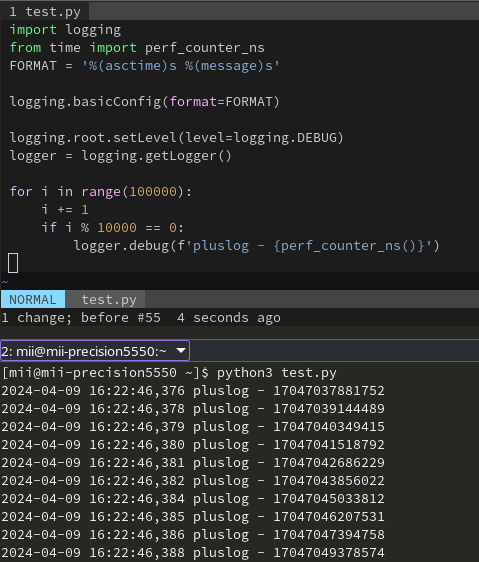
\includegraphics[width=8cm]{figures/introduction/python_log_time}
    \caption{An example of logging being used to find the time after every 10,000 executions of adding to x. Note that
    while the logging library has a time function, there is no way inject higher resolution timers without manually
    calling them. In the output there is also the perf counter, showing a far higher precision output of execution}
    \label{fig:python_log_time}
\end{figure}

\subsubsection{PyTracer}\label{subsubsec:pytracer}
As an alternative to logging, the python sys package includes a settrace module\cite{PythonSystrace} that allows for the
injection of code into individual callbacks of the python interpreter.
This is a powerful tool, as it allows us to analyse individual stack frames, we can use this to analyse executed opcodes
and derive energy usage metrics from predictions of their energy footprint - to understand the opcodes we will need
to make further use of the Disassembler module \textit{dis}\cite{PythonDis}.
Furthermore, these frames contain contextual information that will allow a working profiler to pinpoint areas of
contention to developers.

The major drawback of tracing is similar to logging, as any form of tracing is invasive, and will skew results, this can
be mitigated if the footprint of the tracer is known and accounted for in the final results.

\begin{figure}[H]
    \centering
    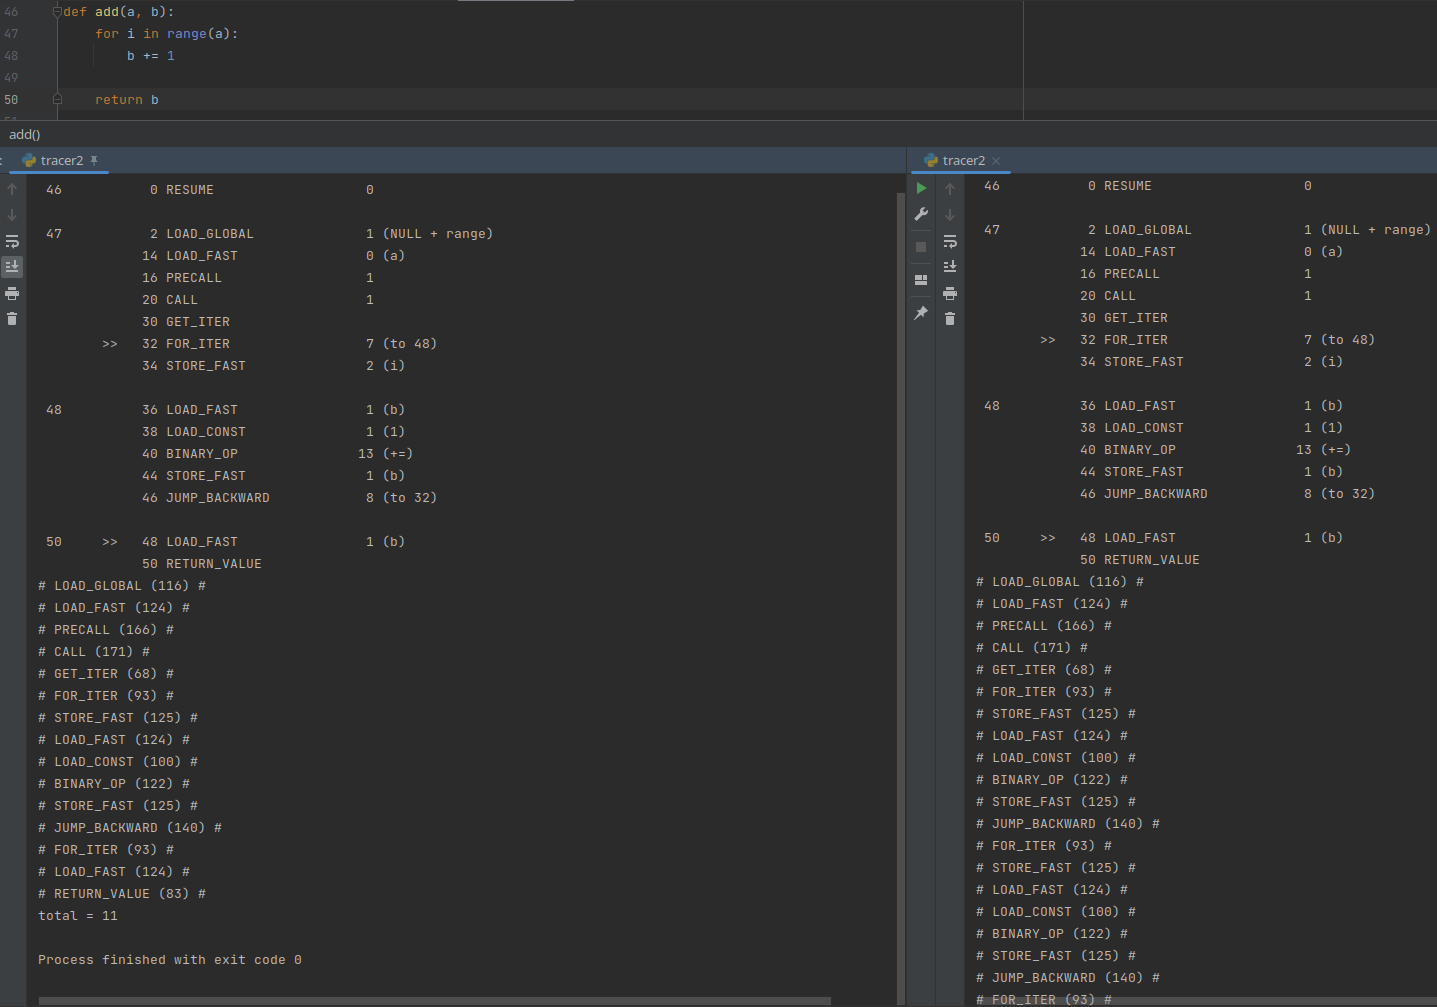
\includegraphics[width=12cm]{figures/introduction/tracer_example}
    \caption{An example of using pytracer to trace the execution of a function that adds two values via iterating over
    the first, the output at the bottom is split into calling \texit{add(1, 10)} (left) and \textit{add(2, 10)} (right),
    first the bytecode of the function is printed using the diassembler module (with line numbers on the far left),
        followed by the individual opcodes being run - note that the output on the right is identical except for the
    repeated opcodes in the output on the right.}
    \label{fig:pytracer_example}
\end{figure}


\subsubsection{Control}
Before beginning experiments, we first must test baseline values that will contextualise our results later on.

\chapter{Tests}\label{ch:tests}

\section{Bash Time}\label{sec:bash-time}
The first profiling method we will test is simply bash time, the assumption to make for this section is that the energy
profile can be accurately predicted by simply knowing the amount of time a process has spent in real, user, and kernel
time.

\subsubsection{Internal Consistency}
The first step in our process is to verify that running an algorithm multiple times remains consistent in terms of the
amount of energy used over the time taken.
From the previous section, it is clear that there is a large amount of variance in time taken for algorithms to complete
- this section seeks to prove that the variance of time predictably scales with the variance of energy usage.
If we can prove that the energy usage of an algorithm is consistent over multiple runs, this would suggest that time
measurements are a required component of predicting energy usage.

\subsubsection{Naive Prediction}
The first step in our process will be to test how reliable simply timing a process is.
As covered in~\ref{subsubsec:bash_time}, bash time provides three values for real, user, and sys time, for the naive
approach we will attempt to take the overall energy usage of the application, and then split it into a ratio of each of
these values - real time encompasses both usr and sys time, so the remaining value for the ration will be the difference
between the summed time in the CPU and the real time (for example, if an application takes 1 second of real time, and
has 0.4 seconds of usr and sys time, the ratio would be 0.2:0.4:0.4).



\section{Opcode Tracing}\label{sec:opcode-tracing}
As purely looking at CPU time doesn't appear to be a reliable method of predicting energy usage, we will now attempt to
look at the opcodes being executed by each script to see if a conclusion can be drawn between executed opcodes and
energy usage.
We have already noted that opcodes can be retrieved by using the sys module, unfortunately there does not appear to be
a process that can also retrieve the operands provided, which have been suggested to affect energy usage, but possibly
not by a significant amount~\cite{OperandPower}

\subsubsection{Opcode Gathering}
In the exploration of profiling tools~\ref{subsubsec:pytracer} we simply took each opcode and printed it to console.
This is a good start, but fails to gather data in a meaningful way, and will be useless for larger programs that execute
more opcodes.

For testing opcode gathering in this section we will use the nbody algorithm, as it scales easily and has a large number
of operations involved.
The primary problem with any kind of granular tracing is that the operations involved in the trace naturally interfere
with the execution of the script itself, as opcodes increase in amount this becomes a very real problem, as we will see
in following examples.

To begin with, we will test
\chapter{Conclusion}\label{ch:conclusion}

\section{Conclusion}\label{sec:conclusion}
\chapter{Conclusion}\label{ch:conclusion}

\section{Conclusion}\label{sec:conclusion}
\chapter{Conclusion}\label{ch:conclusion}

\section{Conclusion}\label{sec:conclusion}
\input{sections/chapters/conclusion/conclusion}

\section{Threats to Validity}\label{sec:threats-to-validity}
\input{sections/chapters/conclusion/threat_to_validity}

\section{Future Work}\label{sec:future-work}
\input{sections/chapters/conclusion/future_work}

\section{Threats to Validity}\label{sec:threats-to-validity}
\input{sections/chapters/conclusion/threat_to_validity}

\section{Future Work}\label{sec:future-work}
\input{sections/chapters/conclusion/future_work}

\section{Threats to Validity}\label{sec:threats-to-validity}
\input{sections/chapters/conclusion/threat_to_validity}

\section{Future Work}\label{sec:future-work}
\input{sections/chapters/conclusion/future_work}
%\cite{Madsen2010}
\printbibliography[heading=bibintoc]
\end{document}